\documentclass[a4paper,english,12pt]{article}
\usepackage{%
	amsmath,%
	amsfonts,%
	amssymb,%
	amsthm,%
	hyperref,%
	url,%
	latexsym,%
	epsfig,%
	graphicx,%
	psfrag,%
	subfigure,%	
	color,%
	tikz,%
	pgf,%
	pgfplots,%
	pgfplotstable,%
	pgfpages,%
	proofs%
}

\usepgflibrary{shapes}
\usetikzlibrary{%
  arrows,%
	backgrounds,%
	chains,%
	decorations.pathmorphing,% /pgf/decoration/random steps | erste Graphik
	decorations.text,%
	matrix,%
  positioning,% wg. " of "
  fit,%
	patterns,%
  petri,%
	plotmarks,%
  scopes,%
	shadows,%
  shapes.misc,% wg. rounded rectangle
  shapes.arrows,%
	shapes.callouts,%
  shapes%
}

\theoremstyle{plain}
\newtheorem{thm}{Theorem}[section]
\newtheorem{lem}[thm]{Lemma}
\newtheorem{prop}[thm]{Proposition}
\newtheorem{cor}[thm]{Corollary}

\theoremstyle{definition}
\newtheorem{defn}[thm]{Definition}
\newtheorem{conj}[thm]{Conjecture}
\newtheorem{exmp}[thm]{Example}
\newtheorem{assum}[thm]{Assumptions}

%\theoremstyle{remark}
\newtheorem{rem}{Remark}
\newtheorem{note}{Note}

\makeatletter
\def\th@plain{%
  \thm@notefont{}% same as heading font
  \itshape % body font
}
\def\th@definition{%
  \thm@notefont{}% same as heading font
  \normalfont % body font
}
\makeatother
\date{}
%\usepackage[utf8x]{inputenc}
%\usepackage[pdftex]{graphicx}

\graphicspath{{./Figures/}}
%opening
\title{ Lecture 3: Sets}
\author{}
\begin{document}
\maketitle

\section{Sets}
Logic is built on set of axioms that are assumed true. Euclid attempted to use the axiomatic constructions for Geometry in his book ``The Elements''. Hilbert formalized Euclidean Geometry in 1899, with a complete set of axioms. 

Set theory is starting place for all rigorous mathematics. It was developed formally by Georg Cantor in lat 19th century. We would develop set theory informally in this lecture. We would provide a glimpse of formal set theory developed from an axiomatic system at the end of the lecture. 
\subsection{Basic Definitions.}
We have an undefined term \textbf{set}, which will informally think of as a collection of objects. Objects contained in the set are called the \textbf{elements} or \textbf{members} of the set. If ${A}$ is a set, and $a$ is an element of the set ${A}$, we write $a\in {A}$. If $a$ is not contained in ${A}$, then we write $a\notin{A}$. 

\textbf{Axiom:} Given any set $A$ and any object $a$, we assume that precisely one of $a \in A$ or $a \notin A$ holds.\\
\textbf{Representation:} A set is written as $\{a,b,c,d\}$, here ordering is irrelevant. 

\begin{defn}[Important sets]
\begin{enumerate}
 \item Set of \textbf{natural numbers} is denoted by $\mathbbm{N} =\{1,2,\ldots\}$.
 \item Set of \textbf{integers} is denoted by $\mathbbm{Z} =\{\ldots,-2,-1,0, 1,2,\ldots\}$.
 \item Set of\textbf{rational numbers}, denoted by $\mathbbm{Q}$, is set of fractions.
 \item Set of \textbf{real numbers} is denoted by $\mathbbm{R}$.
 \item Set of \textbf{whole numbers}, denoted by $\mathbbm{N}_0$, also called set of non-negative integers.
 \item Set with no elements is an \textbf{empty set}, denoted by $\emptyset$.
\end{enumerate}
\end{defn}

\begin{exmp} Let $S=\{n\in \mathbbm{Z}| n \text{ is a perfect square}\}$, then 
\begin{align*}
 S&=\{n\in \mathbbm{Z}| n =k^2\text{ for some} k\in \mathbbm{Z}\},\\
  &=\{n\in \mathbbm{Z}| \text{ is a perfect square } k\in \mathbbm{Z} \text{ such that } n=k^2 \}.
\end{align*}
Notice that $n$ and $k$ are dummy variables in this set notation.
\end{exmp}

\begin{defn}[Intervals] Let $a,b$ be real numbers.
\begin{itemize}
\item An \textbf{open bounded interval} is defined as 
	\begin{equation*}
		(a,b) \triangleq \{x\in \mathbbm{R}: a<x<b\}.
	\end{equation*}
\item A \textbf{closed bounded interval} is defined as 
	\begin{equation*}
	[a,b]:= \{x\in \mathbbm{R}: a\leq x\leq b\}.
	\end{equation*}
\item A \textbf{half-open interval} is defined as 
	\begin{equation*}
	[a,b):= \{x\in \mathbbm{R}: a<x\leq b.
	\end{equation*}
\item An \textbf{open unbounded interval} is defined as 
	\begin{equation*}
	(a,\infty):= \{x\in \mathbbm{R}: a< x\}.
	\end{equation*}
\item A \textbf{closed unbounded interval} is defined as 
	\begin{equation*}
	[a,\infty):= \{x\in \mathbbm{R}: a\leq x \}.
	\end{equation*}
%\item An \textbf{infinite interval} is defined as $[a,\infty):= \{x\in \mathbbm{R}: a\leq x\}$. Other infinite intervals can be $(a,-\infty)$, $(-\infty,b]$, $(-\infty,\infty)=\mathbbm{R}$.
\end{itemize}
\end{defn}

\begin{rem}$+\infty$ and $-\infty$ are not real numbers.
\end{rem}
\begin{rem}Dummy variables cannot be used outside the definition without redefining them. For example, let $y \in [a,b]$, then $y \geq a$ and $y \leq b$.
\end{rem}

\subsection{Relation between Sets}
We are interested in finding relations between sets.
\begin{defn}[Subset] Let ${A}$ and ${B}$ be sets. We say that ${A}$ is a \textbf{subset} of ${B}$ if $x\in {A}$ implies $x\in {B}$, and is denoted by ${A}\subseteq {B}$. If $A$ is not a subset of $B$, we write $A \nsubseteq B$.
\end{defn}
This is shown in the Figure~\ref{Fig:Sets}
\begin{figure}[!h]
\centering
 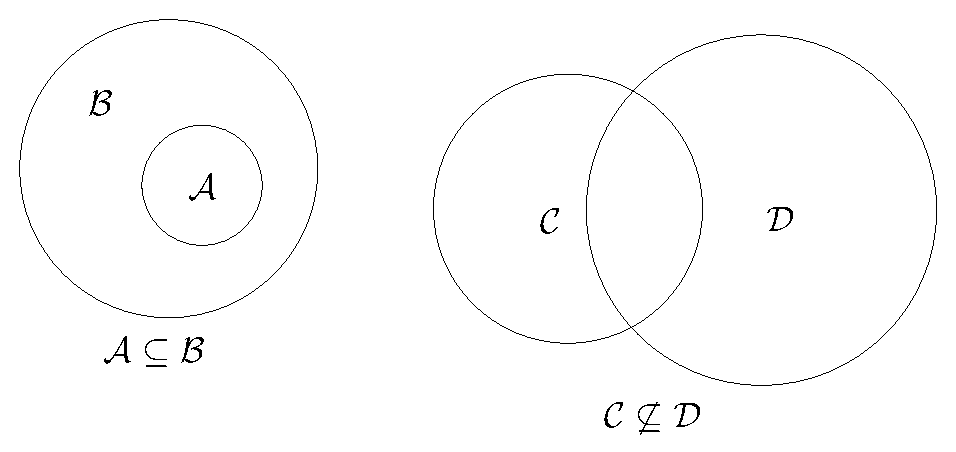
\includegraphics[height=2.0in]{fig33.eps}
\caption{In first example, $A \subseteq B$. In second example, $C \nsubseteq D$.}
\label{Fig:Sets}
\end{figure}
In other words, we can say that ${A}\subseteq {B}$ if $\forall x ([x\in {A}] \rightarrow [x\in{B}])$. While, we say that ${A}\nsubseteq{B}$ if $(\exists x) ([x\in{A}]\wedge[x\not\in{B}])$.

\begin{lem} Let ${A},{B}$, and ${C}$ be sets, then the following are true.
\begin{enumerate}
 \item ${A}\subseteq {A}$.
 \item ${\emptyset}\subseteq{A}$.
 \item If ${A}\subseteq{B}$ and ${B}\subseteq{C}$ then ${A}\subseteq{C}$.
\end{enumerate}
\end{lem}

\begin{proof} Let ${A},{B},$ and ${C}$ be sets.
\begin{enumerate}
 \item %Since $\forall x\in{A}$ implies $x\in{A}$. This implies ${A}\subseteq {A}$. Alternatively, 
Let $x$ be an arbitrary element of set ${A}$. Since any element in ${A}$ is in ${A}$ itself, therefore ${A}\subseteq {A}$.
 \item We need to show that for any $x \in \emptyset$, we have $x \in A$. However, since empty set $\emptyset$ has no elements, conclusion necessarily follows. %Let $x \in \emptyset$, then Since $\forall x \in {\emptyset}$ implies $ x \in {A}$
 \item Let's assume ${A}\subseteq {B}$ and $B \subseteq C$. Let $x$ be an arbitrary element of set ${A}$, then by assumption $A \subseteq B$, we have $x \in {B}$. Further, since ${B}\subseteq{C}$, we have $x\in {C}$. Since choice of $x$ was arbitrary in $A$, we conclude? ${A}\subseteq{C}$.
\end{enumerate}
\end{proof}

\begin{defn}[Equality of Sets] Let ${A}$ and ${B}$ sets. We say that ${A}$ equals ${B}$, denoted ${A}={B}$, if ${A}\subseteq {B}$ and ${B}\subseteq {A}$. 
\end{defn}
To show $A=B$, we would show $A \subseteq B$ and $B \subseteq A$. To show $A \subseteq B$, we would choose arbitrary $a \in A$, and logically deduce that $a \in B$. Similarly, to show $B \subseteq A$, we would choose arbitrary $b \in B$ and logically deduce that $b \in A$.
\begin{defn}[Proper Subset] We say that ${A}$ is a proper subset of ${B}$ if ${A}\subset {B}$, and ${A}\neq {B}$, denoted as ${A}\varsubsetneq {B} ({A}\subset {B})$.
\end{defn} 
\begin{lem} Let ${A},{B},$ and ${C}$ be sets, then following is true
\begin{enumerate}
 \item ${A}= {A}$.
 \item If ${A}= {B}$ then ${B}= {A}$.
 \item If ${A}= {B}$ and ${B}= {C}$ then ${A}= {C}$.
\end{enumerate}
\end{lem}
\begin{defn}[Power Set] Let ${A}$ be a set. The \textbf{power set} of ${A}$ denoted by $\mathcal{P}(A)$ is the set whose elements are subsets of ${A}$.
\end{defn}

\begin{exmp}Power set of $S=\{1,2\}$, is ${P}=\{\{1\},\{2\},\{1,2\},\emptyset\}$.
\end{exmp}

\begin{exmp}[Russell's Paradox] Let set $S$ be defined as 
\begin{align*}
S &\triangleq \{\text{ set of all sets}\},\\
T &\triangleq \{{A}\in{S}|{A}\not\in{A} \}.
\end{align*}
Then is $T \in T$? If $T \in T$, then $ T \not\in T$ by definition. If $T \not\in T$, then $T \in T$ by definition.
\end{exmp}
To resolve such paradoxes. Set theory is built from some basic axioms. One such axiomatic system is discussed below.

\section{Axiomatic System for Set Theory}
We will study one of the widely accepted axiomatic system for set theory due to Zermelo and Fraenkel. We would refer to them as ZF axioms. 
Informally we tend to distinguish between sets and elements. In the ZF axioms we make no such distinction. Everything in the ZF axioms is a set. 
Once we assume that everything in the ZF axioms is a set, then the relation of membership, denoted by the symbol $\in$, is a relation between sets. 
\subsection{Zermelo-Fraenkel axioms}
\begin{enumerate}
	\item \textbf{Axiom of Extensionality.} Two sets are equal if they have the same elements. That is,
\begin{equation*}
 \forall x \forall y [\forall z (z\in {x} \Leftrightarrow z\in {y}) \Rightarrow {x}={y}].
\end{equation*}
	\item \textbf{Axiom of Empty Set.} There is a set $z$ such that $x \notin z$ for all sets $x$.
	\item \textbf{Axiom of Pairing.} If ${x}$ and ${y}$ are sets, then there exists a set which contains ${x}$ and ${y}$ as elements. That is,
\begin{equation*}
 \forall x \forall y \exists z (x \in z  \wedge  y\in z).
\end{equation*}
	\item \textbf{Axiom of Union.} The union over the elements of a set exists. Let $x$ be a set. There is a set $z$ such that $w \in z$ if and only if there is some $y \in x$ such that $w \in y$. That is,
\begin{equation*}
 \forall x \exists z \forall w [(w \in y  \wedge  y \in x) \Rightarrow w \in z].
\end{equation*}
	\item \textbf{Axiom of Power Set.} Let ${x}$ be a set. There is a set $z$ such that $w \in z$ if and only if
$w \subseteq x$. That is,
\begin{equation*}
 \forall x \exists y \forall z [(z \subseteq x) \Rightarrow z \in y].
\end{equation*}
	\item \textbf{Axiom of Regularity.} Every non-empty set ${x}$ contains a member ${y}$ such that
 ${x}$ and ${y}$ are disjoint sets. That is,
\begin{equation*}
 \forall x [\exists a (a \in x) \Rightarrow \exists y (y \in x \wedge \neg \exists z(z \in y \wedge z \in x))].
\end{equation*}
	\item \textbf{Axiom Schema of Specification/Separation/Restricted Comprehension.} Let $P(y)$ be a logical property of sets with one free variable $y$ that can be formulated in the context of the ZF axioms. Let ${x}$ be a set. Then
there is a set ${z}$ such that $y \in{z}$ if and only if $y \in {x}$ and $P(y)$ is true.

	\item \textbf{Axiom Schema of Replacement.} Image of any set $x$ under any definable function $f:x \to y$ will also fall inside a set $z$. Let $f(s, t)$ be a functional property of sets with two free variables $s$ and $t$  that can be formulated in the context of the ZF axioms. Let ${x}$ be a set. Then there is a set ${z}$ such that $y\in {z}$ if and only if there is some $w \in {x}$ such that $f(w, y)$ is true.
	
 \item \textbf{Axiom of Infinity.} There exists a set having infinity many elements. Let's define $s(w) = w \cup \{w\}$ for any set $w$. Then, there is a set ${x}$ such that $\emptyset  \in {x}$, and if ${y} \in {x}$ then $s(y) \in {x}$. Formally,
\begin{equation*}
 \exists x [\emptyset \in x \wedge \forall y ( y \in x \Rightarrow s(y) \in x)].
\end{equation*}

\item \textbf{Axiom of Choice.} Let $x$ be a set. Suppose that if y$,w \in x$, then $y \neq \emptyset$ and $y\cap w = \emptyset$. Then there is a set $z$ such that if $y \in x$, then $y\cap z$ contains a single element. %For any set ${x}$, there is a binary relation $R$, which well-orders ${x}$. This means $R$ is a linear order on ${x}$ such that every non-empty subset of ${x}$ has a member which is minimal under $R$. That is, $\forall {x}\exists R $($R$ well-orders ${x}$)
 \end{enumerate}


\end{document}
